\documentclass[11pt]{article}
\usepackage[utf8]{inputenc}
%\usepackage[latin1]{inputenc}
\usepackage[spanish]{babel}
\decimalpoint
\usepackage{anysize}
\usepackage{graphicx} 
\usepackage{amsmath}
\usepackage{booktabs}
\usepackage{tabulary}
\usepackage{nccmath}
\usepackage{float}
\usepackage{tikz}
\usetikzlibrary{patterns}
\usetikzlibrary{decorations.markings}
\usepackage{pgfplots}
\usepackage{etex}
\usepackage{color}
\usepackage{listings}
\renewcommand{\arraystretch}{1.5}
\lstset{ %
language=Python,                % choose the language of the code
basicstyle=\normalsize,       % the size of the fonts that are used for the code
numbers=left,                   % where to put the line-numbers
numberstyle=\footnotesize,      % the size of the fonts that are used for the line-numbers
stepnumber=1,                   % the step between two line-numbers. If it is 1 each line will be numbered
numbersep=5pt,                  % how far the line-numbers are from the code
backgroundcolor=\color{white},  % choose the background color. You must add \usepackage{color}
showspaces=false,               % show spaces adding particular underscores
showstringspaces=false,         % underline spaces within strings
showtabs=false,                 % show tabs within strings adding particular underscores
frame=single,   		% adds a frame around the code
tabsize=4,  		% sets default tabsize to 2 spaces
captionpos=b,   		% sets the caption-position to bottom
breaklines=true,    	% sets automatic line breaking
breakatwhitespace=false,    % sets if automatic breaks should only happen at whitespace
escapeinside={\#}{)}          % if you want to add a comment within your code
}
\marginsize{1.5cm}{1.5cm}{1cm}{2cm}  
\title{Tarea de diferenciación numérica. \\ Curso de Física Computacional}
\author{M. en C. Gustavo Contreras Mayén}
\date{ }
\begin{document}
\maketitle
\fontsize{14}{14}\selectfont
\begin{enumerate}
\item Usando una aproximación por diferencias finitas de orden $O(h^{2})$, calcula $f'(2.36)$ y $f''(2.36)$, a partir de los datos:
\begin{center}
\begin{tabular}{c | c | c | c | c}
x & 2.36 & 2.37 & 2.38 & 2.39 \\ \hline
f(x) & 0.85866 & 0.86289 & 0.86710 & 0.87129
\end{tabular}
\end{center}
\item Dados los siguientes datos
\begin{center}
\begin{tabular}{c | c | c | c | c | c }
x & 0.84 & 0.92 & 1.00 & 1.08 & 1.16 \\ \hline
f(x) & 0.431711 & 0.398519 & 0.367879 & 0.339596 & 0.312486
\end{tabular}
\end{center}
Calcula $f''(1)$ con la mayor precisión posible.
\item La palanca AB de longitud $R=90$ mm está girando con velocidad angular constante $d\theta/dt= 5000$ rev/min.
\begin{center}
\begin{tikzpicture}[font=\small, scale=1.4, fill=]
\draw (-0.4,-0.3) [pattern= north east lines] rectangle (0.6,0);
\draw (-0.1,0) -- node [above left]{A} (-0.1,0.3)arc (180:0:0.2cm) -- (0.3,0);
\draw (0.1,0.3) circle (0.05);
\draw [dashed] (0.1,0.3) -- node [midway, below] {x} (3.3,0.3);
\draw (3.3,0.3) circle (0.05);
\draw (1.15,1.45) circle (0.05);
\draw (0.1,0.49) -- node [midway, above] {R}(1,1.42);
\draw (0.27,0.4) -- (1.18,1.32);
\draw (1,1.42) -- (3.35,0.15) [rotate=-120] arc  (0:180:0.1cm);
\draw (3.47,0.31) -- node[midway, above, sloped]{2.5R}(1.1,1.6) [rotate=60] arc (0:180:0.1cm);
\draw (1,1.9) node {B};
\draw (2.8,-0.2) [pattern= north east lines] rectangle (4.5,-0.1);
\draw (3.05,0.65) [pattern= north east lines] rectangle (4.5,0.55);
\draw [thick] (3.1,0.3) -- (3.1,-0.07) -- (4.3,-0.07) -- node [midway, right]{C}(4.3,0.55) -- (3.1,0.55);
\draw [thick] (3.8,-0.07) -- (3.8,0.55);
\draw [thick] (3.9,-0.07) -- (3.9,0.55);
\draw [thick] (4,-0.07) -- (4,0.55);
\draw (0.5,0.3) arc (0:70:0.2cm);
\draw (0.7,0.5) node {$\theta$};
\end{tikzpicture}
\end{center}
La posición del pistón C como se muestra, varía con el ángulo $\theta$
\[x = R \left( \cos \theta + \sqrt{2.5^{2} - \sin^{2} \theta} \right)\]
Escribe un programa en python que calcule mediante diferenciación numérica la aceleración del pistón en $\theta= 0^{\circ}, 5^{\circ}, 10^{\circ},\ldots, 180^{\circ}$.
\item Las estaciones de radar \textit{A} y \textit{B} están separadas por una distancia $a=500$ m; rastrean el avión \textit{C} registrando los ángulos $\alpha$ y $\beta$ en intervalos de un segundo. Si hay tres lecturas sucesivas
\begin{center}
\begin{tabular}{c l l l }
t(s) & 9 & 10 & 11 \\ \hline
$\alpha$ & $54.80^{\circ}$ & $54.06^{\circ}$ & $53.34^{\circ}$ \\ \hline
$\beta$ & $65.59^{\circ}$ & $64.59^{\circ}$ & $63.62^{\circ}$
\end{tabular}
\end{center}
\begin{figure}[H]
	\centering
	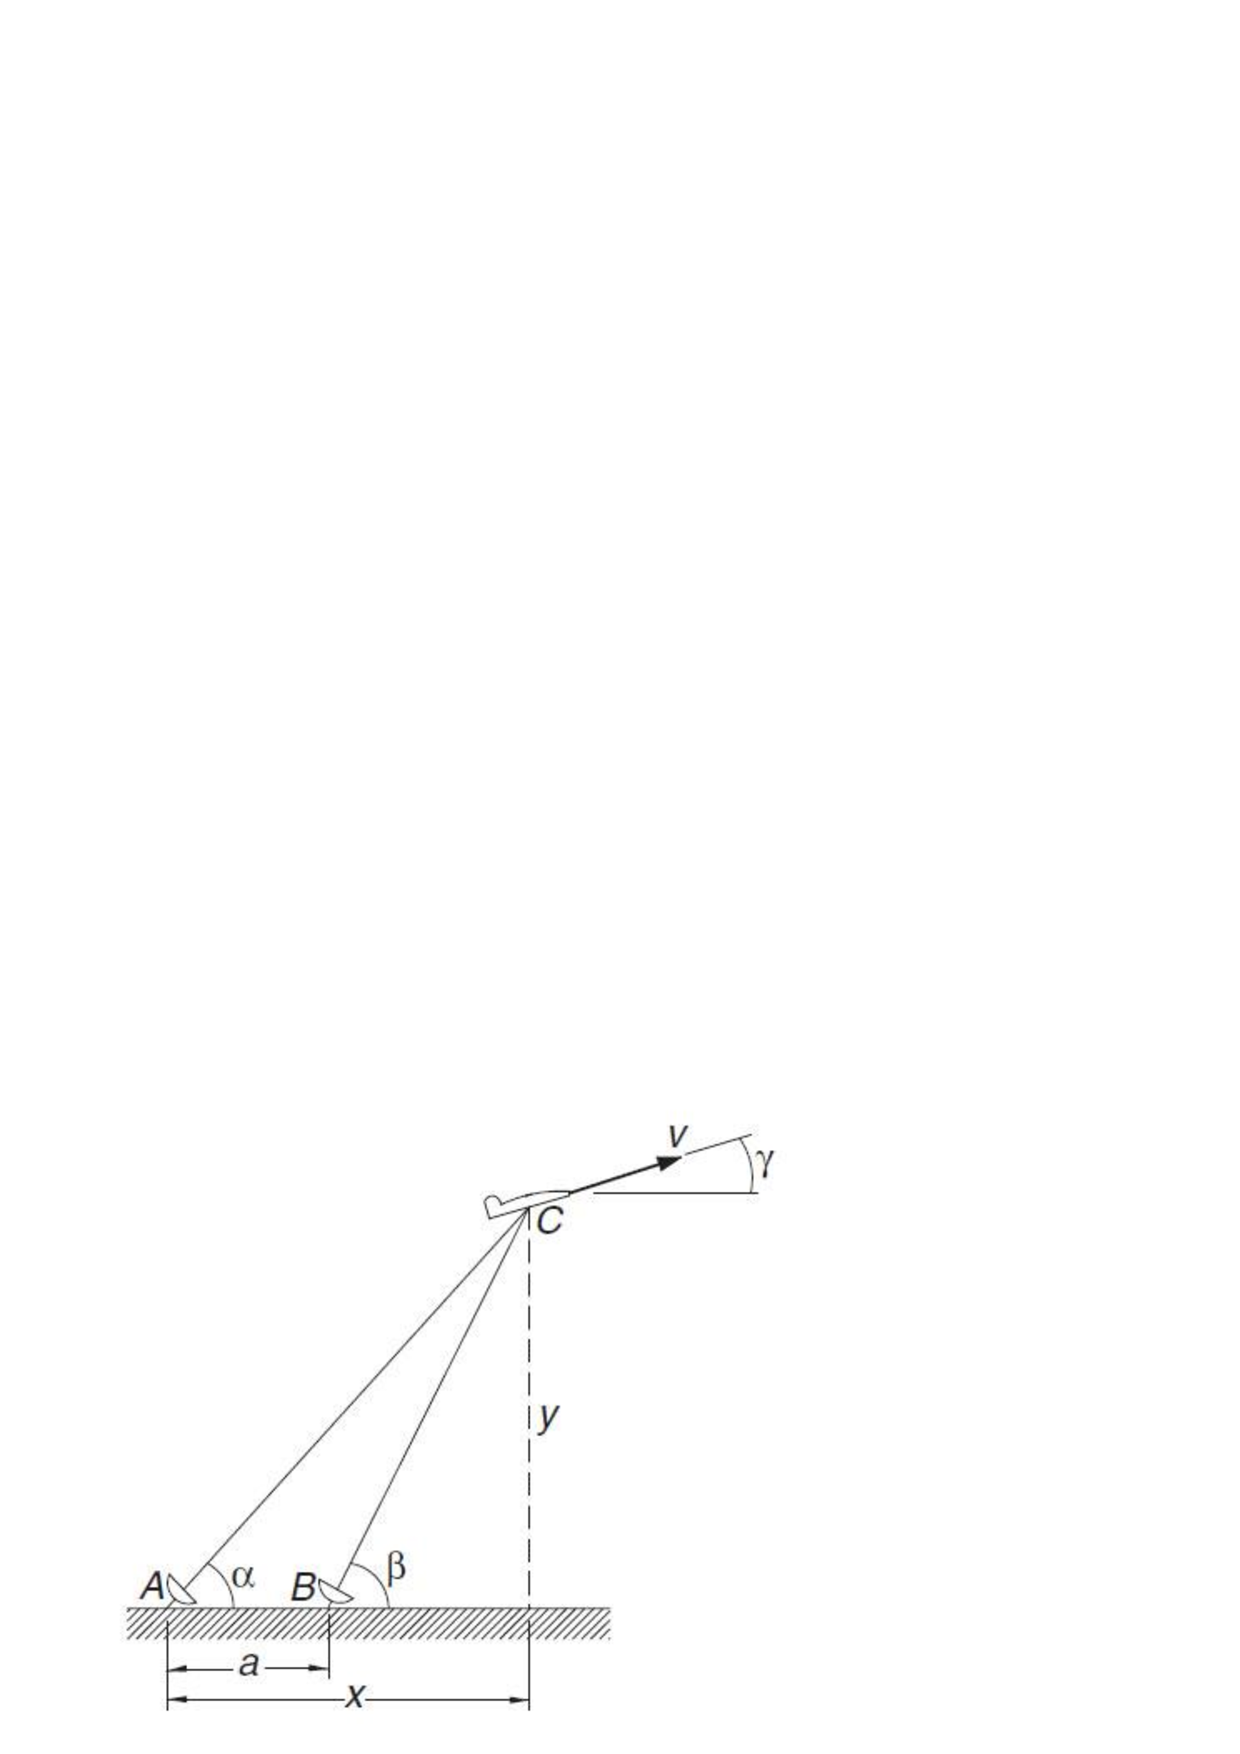
\includegraphics[scale=0.6]{Imagenes/ExamenFinal02_01.jpg} 
	\caption{Estaciones de radar y el avión.}
\end{figure}
Calcula la velocidad $v$ del avión y el ángulo de subida $\gamma$ en $t=10$ segundos. Las coordenadas del avión las tomamos de
\[x = a \dfrac{\tan \beta}{tan \beta - tan \alpha} \hspace{1.5cm} y= a\dfrac{tan \alpha \tan \beta}{\tan \beta - \tan \alpha}\]
\item Obtén la aproximación por diferencias centrales de $f''(x)$ de orden $O(h^{4})$ aplicando la extrapolación de Richardson a la aproximación por diferencias centrales de orden $O(h^{2})$.
\item Obtén la primera aproximación por diferencias centrales para $f^{4}(x)$ a partir de la serie de Taylor.
\end{enumerate}
\end{document}